\documentclass[10pt,conference]{IEEEtran}
\usepackage[T1]{fontenc}
\usepackage{cite}
\usepackage{amsmath}
\usepackage{graphicx}
\usepackage[hidelinks]{hyperref}
% ICSE 2027 Tool Demonstration and Data Showcase: author-free working draft.
% Restore the agreed author list for single-anonymous submission.
% TODO: add the demonstration video URL at the end of the abstract.
\hypersetup{pdfauthor={}}
% Generated from TrustSECO scoring/policy.json; do not edit by hand.
\newcommand{\TrustPolicy}{trust-v2.0.0}
\newcommand{\TrustCoverage}{80}
\newcommand{\TrustFreshness}{24}
\newcommand{\TrustHistory}{7}
\newcommand{\TrustRecovery}{1}
\newcommand{\TrustWeights}{0.35,0.25,0.2,0.1,0.05,0.05}
\newcommand{\TrustReferences}{50,15552000,100,63072000,5000,0.05}
\newcommand{\TrustMultipliers}{1,0.95,0.85,0.5,0.25}
\newcommand{\TrustHighCap}{49}
\newcommand{\TrustCriticalCap}{24}
\newcommand{\TrustExploitedCap}{9}

\begin{document}
\title{TrustSECO: Building Software Trust through Community-Verified Evidence}
\author{\IEEEauthorblockN{Anonymous Authors}}
\maketitle

\begin{abstract}
Software engineers build on one another's work every day. TrustSECO pursues a community-operated model in which they can also build the evidence that makes this reliance well founded. Contributors collect and sign measurements; the infrastructure records provenance, evaluates agreement, and presents scores alongside supporting evidence. Engineers can inspect, question, and contribute to that evidence. This demonstration follows a dependency assessment through the portal to community verification and accountability. We describe the collection, verification, and scoring model, then outline how package-manager experiments with developers and organizations can test whether shared evidence earns confidence and improves software selection.
\end{abstract}
\begin{IEEEkeywords}
software trust, software ecosystems, community verification, software selection
\end{IEEEkeywords}

\section{Introduction}
A software engineer selecting a dependency must decide whether another project's software is suitable for the system being built. Hou and Jansen define software trust as ``the willingness of SECO actors to accept risks based on subjective beliefs''~\cite[Sec.~4.1.6]{hou2023systematic}. Their definition encompasses expectations of dependable producers and software that performs as intended despite uncertainty. Repository measurements inform these expectations; they do not establish software safety.

Software reuse is an act of confidence in other people's work. TrustSECO pursues a long-standing ambition: to make that confidence something the software engineering community can build together. Engineers should be able to benefit from one another's scrutiny, contribute what they learn, and see why a dependency deserves their trust. Beller and Hejderup's vision of blockchain-based software engineering~\cite{beller2019blockchain} points towards such shared infrastructure. TrustSECO brings this ambition into a working tool: evidence that engineers can inspect, question, and help maintain.

This paper introduces TrustSECO, a community-operated tool that connects signed data collection, community corroboration, an auditable ledger, and an evidence-oriented web portal. Its scores offer an entry point into the underlying measurements. The portal distinguishes a local estimate based on reported observations from a confirmed score based on eligible corroborated evidence whose relevant ledger events have finalized. Missing evidence and unresolved disagreements therefore affect what the system can present as confirmed.

The demonstration follows an engineer from a package overview to its supporting evidence. Whether this model improves decisions or earns justified confidence remains for empirical evaluation.

\section{An Engineer's View of TrustSECO}
\label{sec:workflow}
Trust evidence belongs at the moment a developer adds a dependency. npmSECO already evaluated this approach: it displayed trust information before npm installation and received encouraging usability feedback through interviews with 20 software engineers~\cite{hou2024npmseco}.

Building on that experience, our intended workflow checks a selected version against an organizational threshold. A low score prompts exploration of alternatives or deeper security-team assessment, with blocking determined by policy. This policy integration extends the evaluated approach. The demonstration uses Flask to show the supporting evidence and verification history in the portal.



\begin{figure*}[t]
\centering
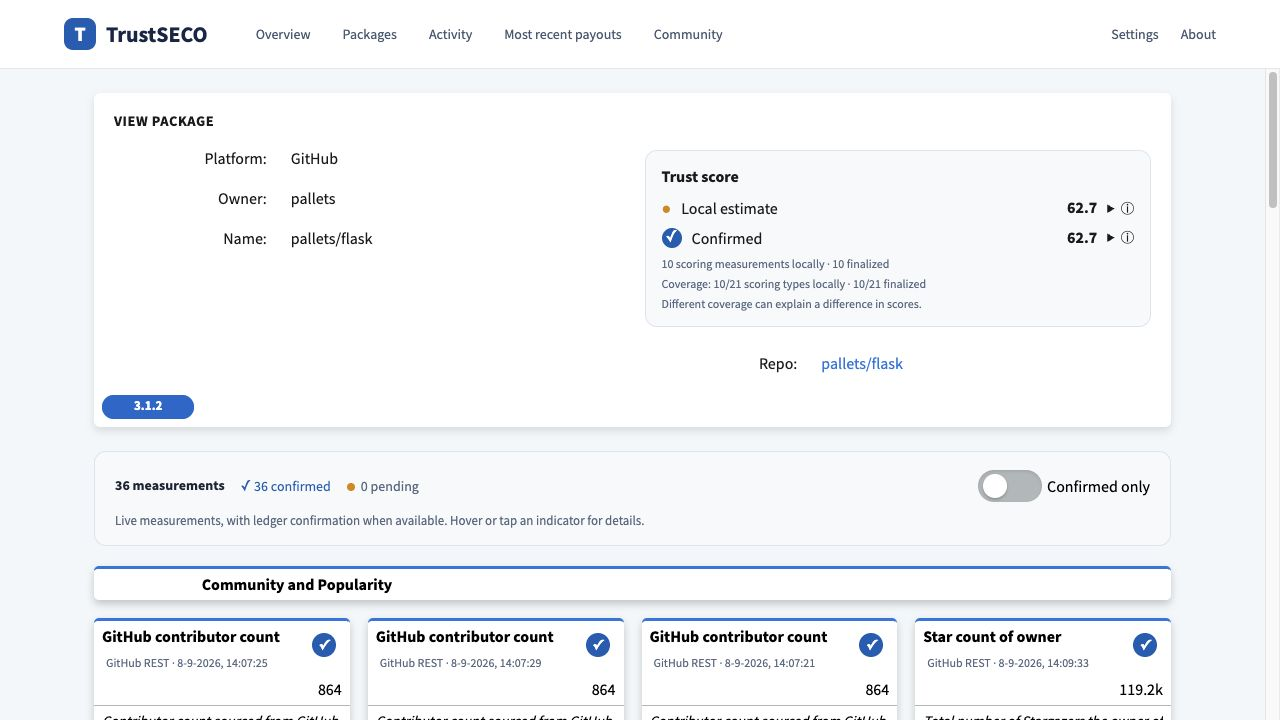
\includegraphics[width=0.72\textwidth]{images/flask-detail-current.png}
\caption{Flask package detail view: local and confirmed scores, evidence coverage, and measurement cards. This interface illustration uses an earlier scoring model; its displayed values do not illustrate the equations presented here.}
\label{fig:flask-detail}
\end{figure*}

\subsection{From a score to its evidence}
The package view (Figure~\ref{fig:flask-detail}) provides a compact summary, while measurement details expose what was reported. A confirmed measurement requires community agreement and ledger finality. An engineer can therefore distinguish an observation that has merely arrived from one that has completed the verification process. Coverage accompanies the score so that a partial set of inputs is not mistaken for a comprehensive assessment.

Measurements describe the repository at observation time. Although they are associated with a package version in the portal, they do not reconstruct the historical state of the repository when that version was released. The demonstration makes this distinction explicit. Similarly, a missing or failed collection is not interpreted as a measured zero.

\subsection{From evidence consumer to contributor}
An engineer can also run a contributor node. Settings guides the user through creating a signing identity, linking its public key to GitHub, requesting admission, and starting collection after approval. Data-source credentials authorize API access and are stored separately from the signing identity. Each submitted observation identifies its contributor, source, method, and time of collection. The community view exposes the resulting rounds and participant standing.

Engineers can thus both inspect and help maintain the evidence supporting dependency decisions.

\subsection{An explicit scoring model}
TrustSECO treats the accumulation and loss of trust differently: positive evidence contributes a bounded baseline, while vulnerabilities affecting the selected version can sharply reduce the score. For a nonnegative measurement $x_i$ and reference $a_i>0$, the baseline is
\begin{equation}
 z_i=\begin{cases}x_i/(x_i+a_i),&\text{higher is better},\\a_i/(x_i+a_i),&\text{lower is better},\end{cases}
 \quad B=100\sum_{i\in I}w_i z_i.
\label{eq:normalization}
\end{equation}
The six indicators are yearly commits, time since latest release, contributors, project age, dependent packages, and Stack Overflow question share. In this order, their weights are $(\TrustWeights)$ and references $(\TrustReferences)$; ages use seconds and question share uses percentage points. Only release recency is lower-is-better. Popularity receives at most 10\% of the budget; raw issues, dependency counts, owner-wide stars, and duplicate contributor counts earn no additional weight. Stack Overflow uses $x/(x+0.05)$: zero maps to zero, 0.05\% maps to 0.5, and increasing values never reverse the contribution.

For distinct applicable advisories $V$, with severity multipliers $m_v$ and ceilings $c_v$, the target and upward recovery rule are
\begin{equation}
\begin{aligned}
 Q_t&=\min\left(B_t\prod_{v\in V}m_v,\;\min(\{100\}\cup\{c_v:v\in V\})\right),\\
 S_t&=\min(Q_t,\;S_{t-1}+\rho\Delta_t),\qquad \rho=\TrustRecovery.
\end{aligned}
\label{eq:score}
\end{equation}
Here $\Delta_t$ is elapsed time in days supported by fresh evidence. A decrease takes effect immediately; recovery is limited to one point per supported day. The \href{https://www.first.org/cvss/v4.0/specification-document}{Common Vulnerability Scoring System (CVSS)} describes vulnerability characteristics and rates their severity. Its none, low, medium, high, and critical categories apply multipliers $(\TrustMultipliers)$; high and critical also cap scores at \TrustHighCap{} and \TrustCriticalCap{}. The U.S. Cybersecurity and Infrastructure Security Agency (CISA) maintains the \href{https://www.cisa.gov/known-exploited-vulnerabilities-catalog}{Known Exploited Vulnerabilities catalog}, which records vulnerabilities exploited in real attacks. An applicable entry caps the score at \TrustExploitedCap{}. With baseline 80, one high-severity advisory gives 40 and one critical advisory gives 20. These are policy examples, not measured safety probabilities.

\href{https://osv.dev/}{Open Source Vulnerabilities (OSV)} aggregates vulnerability advisories across open-source ecosystems. TrustSECO queries it for the exact ecosystem, package, and version; withdrawn records are excluded and aliases are deduplicated. CVSS vectors provide a consistent basis for severity assessment. Unknown severity or incomplete security collection makes the assessment unavailable. Evidence expires after \TrustFreshness{} hours. Weighted coverage $C=\sum_{i\in I}w_i$ must reach \TrustCoverage\%; missing positive inputs yield the baseline range $[B,B+100(1-C)]$, with $Q$ using its lower bound. No score is initialized until \TrustHistory{} days of supported history exist. History follows the project across releases; gaps earn no unsupported recovery. An auditable governance correction can restore a target promptly without bypassing its security ceiling. Local results remain provisional; confirmed results require eligible corroboration and finality. All settings remain heuristics requiring empirical validation.

In the longer term, organizations should be able to adjust the weights to emphasize the characteristics they value most, such as maintenance, security, or ecosystem support. An organization $o$ would apply a versioned weight profile $w_i^{(o)}$ in Equation~\ref{eq:score} to the same shared evidence. The profile should accompany the score so that its interpretation remains reproducible; scores from different profiles need not be directly comparable. Organization-specific configuration is a planned capability, not a feature of the current platform.

\section{Building Trust through Community Verification}
\label{sec:community}
Each time-bounded collection round specifies a repository, version, metric, method, and reward. Contributors submit signed observations; ledger replicas apply a common policy for agreement and review.

\subsection{Accountable participation}
Admission requires a GitHub account at least 180 days old, a published Ed25519 signing key, and a signed request proving possession of the matching private key. A designated governor checks admission and attests that the applicant represents a distinct operator. Duplicate registered account identifiers, keys, and operator identifiers are rejected. Additional nodes using the same identity do not create additional votes.

These controls make admission accountable, but account age and key ownership do not prove that different accounts belong to independent people. TrustSECO therefore relies on the governor's admission review. Its permissioned participation model makes that dependency explicit.

\subsection{Three contributors corroborate a measurement}
Each contributor may submit at most one observation per round. Verification requires at least three eligible contributors whose measurements are pairwise compatible under the metric's tolerance. Exactly one maximal compatible group must exist; competing groups, including overlapping groups, leave the result disputed. The upper median of the agreeing group represents the measurement. For example, the current owner-star metric permits a difference up to the larger of five stars or 2\% of the larger observation. Tolerances are provisional policy choices that accommodate small collection differences and require empirical evaluation.

Two observations cannot satisfy the quorum. Agreement remains provisional while the round is open, and a measurement becomes a confirmed score input only after closure and the required ledger finality. Community corroboration concerns the external measurement; ledger consensus concerns the recorded history. A signature establishes attribution, and agreement establishes consistency under the policy. Neither independently establishes the truth of the upstream source.

TrustSECO accepts observations from any admitted contributor. Its standard miner processes eligible open rounds. Consequently, three colluding contributors could target the same measurement. Random assignment of distinct operators to rounds is being developed separately and is not claimed as a guarantee of this demonstrated baseline.

\subsection{Review, suspension, and appeal}
An outlying observation alone does not establish misconduct. The governor must substantiate an incident against an observation in a closed round, recording evidence, a reason, and a root cause. Under the initial policy, three distinct substantiated incidents within 30 days flag a contributor for review; five suspend participation in verification and reward eligibility. Reports associated with the same root cause or round do not accumulate additional strikes.

Suspension excludes the contributor's observations from supporting current verification results. Appeals, overturned incidents, and explicit reinstatement remain in the audit history. Compromised keys can be revoked. These mechanisms allow the community to respond to unreliable contributions while preserving the record of both the original evidence and subsequent decisions. The thresholds govern reviewed incidents, not the number of observers, and do not infer malicious intent automatically.

\subsection{Funding shared trust evidence}
TrustSECO envisions companies funding the collection and verification of software trust data they need. A company allocates TrustCOIN to measurement requests, and contributors earn rewards by supplying observations that satisfy the community's verification rules. This connects demand for trustworthy software information with the effort required to produce and maintain it. Over time, the resulting evidence could also support other platforms and services.

TrustSECO implements funded rounds and reward distribution. Company purchasing and funding flows have not yet been demonstrated; the mechanism by which companies obtain TrustCOIN remains to be specified.

\section{Implementation and Demonstration}
\label{sec:implementation}
TrustSECO combines a web portal, a coordinator and relay, contributor-side collectors, and a Klayr-based ledger. Contributors retain their signing keys; the relay uses a separate transaction-fee identity. Signed observations include a source URL, timestamp, and response hash. The collection client does not archive full source responses, so the hash alone does not ensure that the original response can later be retrieved.

The ledger evaluates round outcomes, contribution standing, and reward eligibility. The portal reads projections of this state. Confirmed score inputs use closed, currently corroborated rounds whose closure has finalized. A newer disputed round suppresses the previous input for that metric; historical observations remain available. Review events can also change eligibility. The versioned scoring policy separates bounded positive evidence, security penalties, and gradual recovery. We do not interpret the resulting score as a calibrated probability of software safety.

Source code and local setup instructions are available in the project repository.\footnote{\url{https://github.com/SecureSECO/TrustSECO-Next}} The demonstration is organized into three stages:
\begin{enumerate}
\item \textbf{Inspect a dependency.} Open the prepared Flask package page, compare local and confirmed scores, and inspect the available measurements and coverage.
\item \textbf{Follow corroboration.} Trace signed observations through an open round, the three-contributor agreement rule, closure, and finality. Use labelled fixtures to contrast agreement with insufficient or conflicting evidence.
\item \textbf{Inspect accountability.} Show the contribution history and a reviewed-incident scenario, distinguishing an outlier from substantiated incidents, suspension, and appeal.
\end{enumerate}
The scenario is a demonstration plan. Fixture values and simulated contributors must be identified as such, and the final video should use the release accompanying the paper.

\section{Related Work}
The TrustSECO infrastructure builds on earlier work proposing a distributed software trust layer~\cite{hou2021trustseco}. The npmSECO evaluation~\cite{hou2024npmseco} provides prior evidence for presenting trust information during package selection. This demonstration contributes the community verification infrastructure supporting that interaction.

\textbf{Distributed ledgers for software engineering.} Beller and Hejderup's ICSE-NIER vision~\cite{beller2019blockchain} connects distributed infrastructure, incentives, and trust in software engineering services. TrustSECO advances this direction through a working workflow for measurement provenance and community review in dependency assessment.

\textbf{Measuring trust.} Boughton et al.~\cite{boughton2024decomposing} propose decomposing software supply-chain trust into relationships and behaviour-based indicators, questioning the grounding of convenient proxies such as stars. Their work motivates a distinction in TrustSECO: corroborating a measurement does not validate its interpretation as a trust indicator. The portal exposes evidence and coverage, while the choice and weighting of indicators remain subjects for evaluation.

\textbf{Independent verification of packages.} Benedetti et al.~\cite{benedetti2025reproducible} study reproducible packaging across six open-source ecosystems. Their verification of correspondence between build inputs and delivered artifacts complements TrustSECO's repository measurements. Incorporating reproducible-build results would require a dedicated collection and verification policy.

\section{Research Agenda}
The next step is to bring this vision into everyday engineering and learn whether people want to make it their own.

\textbf{Trust in everyday package selection.} We want to revisit an npmSECO-style experiment~\cite{hou2024npmseco} in an open-source package manager, involving both developers and organizations. Does shared evidence make them feel better informed and more confident about dependencies? Do prompts encourage exploration of alternatives? Interviews and configurable weight profiles should reveal what participants value, whether they want to adjust weights, and why. Comparing prompted and unprompted workflows should examine actual choices, replacement suitability, and decision effort alongside these experiences; confidence and switching alone do not establish better decisions.

\textbf{Trust lost and regained.} \emph{``Trust comes on foot, and leaves by horse.''} The scoring model makes this philosophy testable through severity-sensitive penalties, hard ceilings, and evidence-supported recovery. Evaluation must establish whether these settings prompt useful reassessment without unfairly disadvantaging well-maintained projects that disclose vulnerabilities. Known-exploited status is distinct from predicted exploitability; EPSS-based prioritization and deployment-specific reachability remain future work. Controlled tests can check arithmetic and state transitions, but longitudinal and independent-host studies are still needed to validate behavioral effects.

\textbf{Sustainable funding and governance.} Can company-funded requests sustain useful participation without rewarding fabricated agreement or neglecting less-funded packages? Evaluation should cover reward allocation, data freshness, review effort, and appeals. Distributed governance must establish who can adjudicate disputed evidence and sanctions.

\textbf{Broader, reproducible evidence.} How can release-specific measurements and reproducible-build results enter the model? Each requires explicit provenance, freshness, and agreement semantics. Cross-ecosystem experiments should examine evidence retention, reproducibility, and operating costs.

\section{Conclusion}
TrustSECO takes a step towards a software ecosystem in which confidence is earned together. Its working pipeline lets engineers inspect shared evidence and contribute to its verification. The ambition is for this shared practice to become part of everyday software reuse: confidence grounded in what a community can show, question, and improve. Evaluating that promise with developers and organizations is the next step.

\bibliographystyle{IEEEtran}
\bibliography{Ref}
\end{document}
